\documentclass[12pt]{article}
\usepackage[margin=1in]{geometry}

% Start of preamble
%==========================================================================================%
% Required to support mathematical unicode
\usepackage[warnunknown, fasterrors, mathletters]{ucs}
\usepackage[utf8x]{inputenc}

\usepackage[dvipsnames,table,xcdraw]{xcolor} % colors
\usepackage{hyperref} % links
\hypersetup{
	colorlinks=true,
	linkcolor=blue,
	filecolor=magenta,      
	urlcolor=cyan,
	pdfpagemode=FullScreen
}

% Standard mathematical typesetting packages
\usepackage{amsmath,amssymb,amscd,amsthm,amsxtra, pxfonts}
\usepackage{mathtools,mathrsfs,dsfont,xparse}

% Symbol and utility packages
\usepackage{cancel, textcomp}
\usepackage[mathscr]{euscript}
\usepackage[nointegrals]{wasysym}
\usepackage{apacite}

% Extras
\usepackage{physics}  % Lots of useful shortcuts and macros
\usepackage{tikz-cd}  % For drawing commutative diagrams easily
\usepackage{microtype}  % Minature font tweaks
%\usepackage{pgfplots} % plots

\usepackage{enumitem}
\usepackage{titling}

\usepackage{graphicx}

% Fancy theorems due to @intuitively on discord
\usepackage{mdframed}
\newmdtheoremenv[
backgroundcolor=NavyBlue!30,
linewidth=2pt,
linecolor=NavyBlue,
topline=false,
bottomline=false,
rightline=false,
innertopmargin=10pt,
innerbottommargin=10pt,
innerrightmargin=10pt,
innerleftmargin=10pt,
skipabove=\baselineskip,
skipbelow=\baselineskip
]{mytheorem}{Theorem}

\newenvironment{theorem}{\begin{mytheorem}}{\end{mytheorem}}

\newtheorem{corollary}{Corollary}
\newtheorem{lemma}{Lemma}

\newtheoremstyle{definitionstyle}
{\topsep}%
{\topsep}%
{}%
{}%
{\bfseries}%
{.}%
{.5em}%
{}%
\theoremstyle{definitionstyle}
\newmdtheoremenv[
backgroundcolor=Violet!30,
linewidth=2pt,
linecolor=Violet,
topline=false,
bottomline=false,
rightline=false,
innertopmargin=10pt,
innerbottommargin=10pt,
innerrightmargin=10pt,
innerleftmargin=10pt,
skipabove=\baselineskip,
skipbelow=\baselineskip,
]{mydef}{Definition}
\newenvironment{definition}{\begin{mydef}}{\end{mydef}}

\newtheorem*{remark}{Remark}

\newtheorem*{example}{Example}

% Common shortcuts
\def\mbb#1{\mathbb{#1}}
\def\mfk#1{\mathfrak{#1}}

\def\bN{\mbb{N}}
\def \C{\mbb{C}}
\def \R{\mbb{R}}
\def\bQ{\mbb{Q}}
\def\bZ{\mbb{Z}}
\def \cph{\varphi}
\renewcommand{\th}{\theta}
\def \ve{\varepsilon}
\newcommand{\mg}[1]{\| #1 \|}

% Often helpful macros
\newcommand{\floor}[1]{\left\lfloor#1\right\rfloor}
\newcommand{\ceil}[1]{\left\lceil#1\right\rceil}
\renewcommand{\qed}{\hfill\qedsymbol}
\renewcommand{\ip}[2]{\langle #1, #2 \rangle}
\newcommand{\seq}[2]{\qty(#1_#2)_{#2=1}^{\infty}}

% Sets
\DeclarePairedDelimiterX\set[1]\lbrace\rbrace{\def\given{\;\delimsize\vert\;}#1}

% End of preamble
%==========================================================================================%

% Start of commands specific to this file
%==========================================================================================%

\usepackage{braket}
\newcommand{\Z}{\mbb Z}
\newcommand{\gen}[1]{\left\langle #1 \right\rangle}
\newcommand{\nsg}{\trianglelefteq}

%==========================================================================================%
% End of commands specific to this file

\title{Math 504 HW1}
\date{\today}
\author{Rohan Mukherjee}

\begin{document}
	\maketitle
	\begin{enumerate}[leftmargin=\labelsep]
		\item Let $e_1, e_2$ both be identity elements of a group $G$. Then, $e_1 = e_1e_2 = e_2$, since we have by definition that $e_1x = xe_1 = x$ for all $x \in G$. Similarly, let $a \in G$ and $b, c$ both be inverses of $a$. Then, $b = b \cdot (a \cdot c) = (b \cdot a) \cdot c = e \cdot c = c$.
		
		\item \begin{enumerate}
			\item Suppose instead that $n \not \mid m$. Then write $m = bn + r$ for some $1 \leq r < n$. We thus have:
			\begin{align*}
				e = a^m = a^{bn + r} a^{bn} \cdot a^r = e^b \cdot a^r = a^r
			\end{align*}
			But this contradicts the minimality of $n$.
			\item Let $G = \langle a \rangle$ be cyclic, and $H \leq G$. It follows that every element of $H$ is of the form $a^{k}$ for some $k \geq 0$ (Since $H \leq G$). Consider the set $Z = \Set{k \in \Z^+ | a^k \in H}$. If $H$ is the trivial subgroup then we are done, else $Z$ is nonempty and thus has a minimal element $\ell$ by the well ordering principle. We claim that $H = \langle a^\ell \rangle$. Indeed, since $H$ is closed under products, we have $(a^\ell)^n = a^{n \ell} \in H$ for any $n \geq 1$. Suppose instead that $H \not \subset \langle a^\ell \rangle$. Then there is some $m$ not divisible by $\ell$ such that $a^m \in H$. Now write $m = b\ell + r$, with $1 \leq r < l$. Then we have $a^m \cdot a^{-b\ell} = a^r \in H$, but this contradicts the minimality of $\ell$. Thus $H = \langle a^\ell \rangle$, which completes the proof.
			\item Write $G = \gen{a}$. We claim that $\Im{f} = \gen{f(a)}$. First notice that $\Im{f} \supset \gen{f(a)}$, since it contains $f(a)$ and is closed under products. Next, given an element $b \in \Im{f}$, by definition we can write $b = f(g)$ for some $g \in G$, and since $g = a^k$ for some $k \geq 0$, we have $b = f(a^k) = f(a)^k$, which shows that $b \in \gen{f(a)}$, completing the proof.
			\item Since $\Z$ is cyclic, any subgroup is also cyclic by part (b). Thus the only possible subgroups are those of the form $m\Z = \Set{mz | z \in \Z} = \gen{m}$, and since these are all subgroups, we are done.
			\item Since $\Z / m\Z$ is cyclic, all subgroups are of the form $\gen{k}$ for some $k \in \Z / m\Z$. We claim that $|\gen{k}| = m/\gcd(m, k)$. We are looking for the smallest integer $n$ such that $nk$ is a multiple of $m$. Notice that $nk$ is also a multiple of $k$, so if we could find such an $n$ $nk \geq \mathrm{lcm}(m, k) = k \cdot (m / \gcd(m, k))$. So we have that $n \geq m / \gcd(m, k)$. We see that $n = m / \gcd(m, k)$ yields a multiple of $k, m$ since $nk = \mathrm{lcm}(m, k)$, which is a multiple of both $m$ and $k$, which proves the above claim. Up to isomorphism, we just get $\Z / d \Z$ for $d \mid m$ as all the subgroups (by taking $k = m/d$).
		\end{enumerate}
		\item \begin{enumerate}
			\item I claim that $\gen{r^2s} \nsg \gen{s, r^2} \nsg D_8$, but $\gen{r^2s}$ is not normal in $D_8$. Notice that $\gen{s, r^2} = \Set{e, s, r^2, r^2s = sr^2 = r^{-2}s = r^2s}$, so $\gen{s, r^2} \nsg D_8$ since it is a subgroup of index 2. We also see that $\gen{r^2s} = {r^2s, ((r^2)s)^2} = {r^2s, r^2sr^2s = r^2ssr^{-2} = e}$, which is another subgroup of index 2 so is normal in $\gen{s, r^2}$. However, $r (r^2s)r^{-1} = r^3sr^3 = s$, which is not in $\gen{r^2s}$, which proves the claim.
			
			\item We see that $\Z/6 = \gen{1}$, which is obviously minimal. I claim that $\Set{2, 3}$ is also minimal. First notice that $\gen{2, 3}$ contains $3 - 1$ so $\Z/6 = \gen{1} \subset \gen{2, 3}$, so it is indeed a generator. However, $\gen{2} = \Set{0, 2, 4}$, and $\gen{3} = \Set{0, 3}$, neither of which are the whole group, so $\Set{2,3}$ is indeed minimal.
			
			\item We see that $\Z \times \Z = \gen{(1, 0), (0,1)}$.
		\end{enumerate}
		\item If we plug $b = c = e$, we get,
		\begin{align*}
			a * d = (a \circ e) * (e \circ d) = (a * e) \circ (e * d) = a \circ d
		\end{align*}
		Which shows they coincide. With this knowledge, if we plug in $b = e$, we get,
		\begin{align*}
			a * (c * d) = (a * c) * d
		\end{align*}
		Finally, if we plug in $a = d = e$, we get $b * c = c * b$.
		
		\item \begin{enumerate}
			\item Notice that $(0, (1, 0, 0))(0, (0, 1, 0)) = (0, (1, 0, 0) \times (0, 1, 0)) = (0, (0, 0, 1))$ while $(0, (0, 1, 0))(0, (1, 0, 0)) = (0, (0, 0, -1))$, so the operation isn't commutative. We see that
			\begin{align*}
				&((a, u)(b, v))(c, w) = (ab-u \cdot v, av + bu + u \times v)(c,w) \\
				&= (abc - c \cdot u \cdot v - (a \cdot w \cdot v + b \cdot w \cdot u + w \cdot (u \times v)), (ab - u\cdot v)w+c(av+bu+u \times v))
			\end{align*}
			On the other hand, we get
			\begin{align*}
				&(a, u)((b, v)(c, w)) = (a, u)(bc-v\cdot w, bw + cv + v \times w)
				\\ &= (abc - a \cdot v \cdot w - (b \cdot u \cdot w + c \cdot u \cdot v + u \cdot (v \times w), a(bw+cv+ v\times w) +
			\end{align*}
		
			\item We see that if $N((a, u)) = 0$, we must have $a^2=0$ and $|u|^2 = 0$ which occurs iff $a = 0$ and $u = 0$. Thus, if $\alpha, \beta \neq 0$, since $N(\alpha \beta) = N(\alpha)N(\beta) \neq 0$, we have that $\alpha \beta \neq 0$. First, I claim that $(1, 0)$ is the identity. We see that $(a, u)(1, 0) = (a - u \cdot 0, 1 \cdot u + 0 \times u) = (a, u)$. I also claim that if $(a, u) \neq 0$, then the inverse of $(a, u)$ is just $(a/(a^2+|u|^2), -u/(a^2+|u|^2))$. Indeed, 
			\begin{align*}
				(a, u) \cdot (a/(a^2+|u|^2), -u/(a^2+|u|^2)) = \qty(\frac{a^2}{a^2+|u|^2} + \frac{|u|^2}{a^2+|u|^2}, -a\frac{u}{a^2+|u|^2} + a\frac{u}{a^2+|u|^2}) = (1, 0)
			\end{align*}
			\item First notice that if $(a, u)$ and $(b, v)$ have integer coefficients, then then $ab - u \times v$ will be the sum / difference of integers and thus also an integer, $av+bu$ will be a vector with integer coefficients, and $u \times v$ will be another vector with integer coefficients just from the formula. Now, if $(a, u)$, $(b, v)$ have norm 1, then the norm of their product is also 1, so this set is closed under products. It is closed under inverses by looking at the inverse formula--$(a/N(\alpha), -u/N(\alpha)) = (a, -u)$. We now consider the ways to get $N(\alpha) = 1$: either $a = \pm 1$ and $u = 0$, or $a = 0$ and $u_1 = \pm 1$, or $u_2 = \pm 1$, or $u_3 = \pm 1$, which gives 8 elements. Visually:
			\begin{align*}
				Q_8 = \Set{(\pm1, 0), \qty(0, \begin{pmatrix} \pm 1 \\ 0 \\ 0 \end{pmatrix}), \qty(0, \begin{pmatrix} 0 \\ \pm 1 \\ 0 \end{pmatrix}), \qty(0, \begin{pmatrix} 0 \\ 0 \\ \pm 1 \end{pmatrix})}
			\end{align*}
		\end{enumerate}
	\end{enumerate}

		\includegraphics[scale=0.75,page=2]{q5.pdf}
		\newpage
		\includegraphics[scale=0.75,page=3]{q5.pdf}
		\newpage
		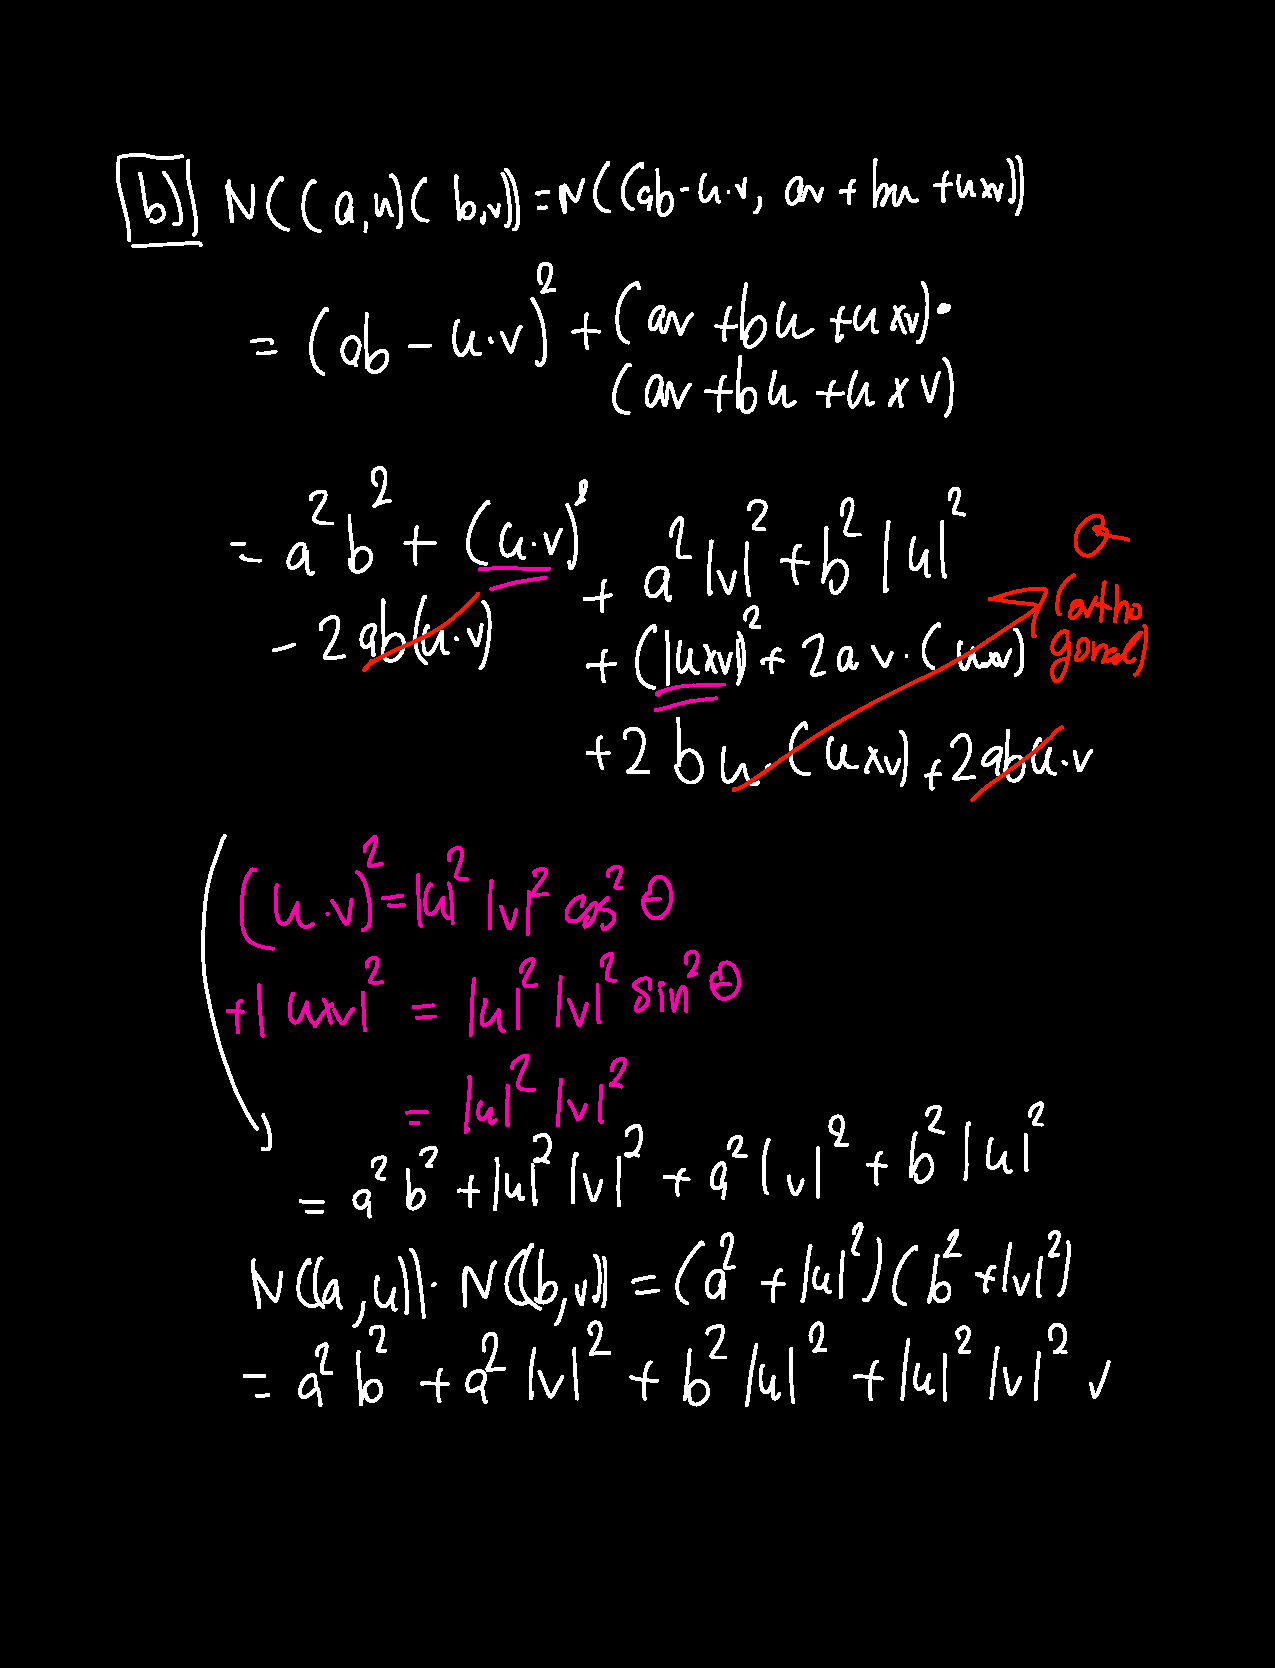
\includegraphics[scale=0.75,page=1]{q5.pdf}
\end{document}
